\documentclass[twoside]{book}

% Packages required by doxygen
\usepackage{fixltx2e}
\usepackage{calc}
\usepackage{doxygen}
\usepackage[export]{adjustbox} % also loads graphicx
\usepackage{graphicx}
\usepackage[utf8]{inputenc}
\usepackage{makeidx}
\usepackage{multicol}
\usepackage{multirow}
\PassOptionsToPackage{warn}{textcomp}
\usepackage{textcomp}
\usepackage[nointegrals]{wasysym}
\usepackage[table]{xcolor}

% Font selection
\usepackage[T1]{fontenc}
\usepackage[scaled=.90]{helvet}
\usepackage{courier}
\usepackage{amssymb}
\usepackage{sectsty}
\renewcommand{\familydefault}{\sfdefault}
\allsectionsfont{%
  \fontseries{bc}\selectfont%
  \color{darkgray}%
}
\renewcommand{\DoxyLabelFont}{%
  \fontseries{bc}\selectfont%
  \color{darkgray}%
}
\newcommand{\+}{\discretionary{\mbox{\scriptsize$\hookleftarrow$}}{}{}}

% Page & text layout
\usepackage{geometry}
\geometry{%
  a4paper,%
  top=2.5cm,%
  bottom=2.5cm,%
  left=2.5cm,%
  right=2.5cm%
}
\tolerance=750
\hfuzz=15pt
\hbadness=750
\setlength{\emergencystretch}{15pt}
\setlength{\parindent}{0cm}
\setlength{\parskip}{3ex plus 2ex minus 2ex}
\makeatletter
\renewcommand{\paragraph}{%
  \@startsection{paragraph}{4}{0ex}{-1.0ex}{1.0ex}{%
    \normalfont\normalsize\bfseries\SS@parafont%
  }%
}
\renewcommand{\subparagraph}{%
  \@startsection{subparagraph}{5}{0ex}{-1.0ex}{1.0ex}{%
    \normalfont\normalsize\bfseries\SS@subparafont%
  }%
}
\makeatother

% Headers & footers
\usepackage{fancyhdr}
\pagestyle{fancyplain}
\fancyhead[LE]{\fancyplain{}{\bfseries\thepage}}
\fancyhead[CE]{\fancyplain{}{}}
\fancyhead[RE]{\fancyplain{}{\bfseries\leftmark}}
\fancyhead[LO]{\fancyplain{}{\bfseries\rightmark}}
\fancyhead[CO]{\fancyplain{}{}}
\fancyhead[RO]{\fancyplain{}{\bfseries\thepage}}
\fancyfoot[LE]{\fancyplain{}{}}
\fancyfoot[CE]{\fancyplain{}{}}
\fancyfoot[RE]{\fancyplain{}{\bfseries\scriptsize Generated by Doxygen }}
\fancyfoot[LO]{\fancyplain{}{\bfseries\scriptsize Generated by Doxygen }}
\fancyfoot[CO]{\fancyplain{}{}}
\fancyfoot[RO]{\fancyplain{}{}}
\renewcommand{\footrulewidth}{0.4pt}
\renewcommand{\chaptermark}[1]{%
  \markboth{#1}{}%
}
\renewcommand{\sectionmark}[1]{%
  \markright{\thesection\ #1}%
}

% Indices & bibliography
\usepackage{natbib}
\usepackage[titles]{tocloft}
\setcounter{tocdepth}{3}
\setcounter{secnumdepth}{5}
\makeindex

% Hyperlinks (required, but should be loaded last)
\usepackage{ifpdf}
\ifpdf
  \usepackage[pdftex,pagebackref=true]{hyperref}
\else
  \usepackage[ps2pdf,pagebackref=true]{hyperref}
\fi
\hypersetup{%
  colorlinks=true,%
  linkcolor=blue,%
  citecolor=blue,%
  unicode%
}

% Custom commands
\newcommand{\clearemptydoublepage}{%
  \newpage{\pagestyle{empty}\cleardoublepage}%
}

\usepackage{caption}
\captionsetup{labelsep=space,justification=centering,font={bf},singlelinecheck=off,skip=4pt,position=top}

%===== C O N T E N T S =====

\begin{document}

% Titlepage & ToC
\hypersetup{pageanchor=false,
             bookmarksnumbered=true,
             pdfencoding=unicode
            }
\pagenumbering{alph}
\begin{titlepage}
\vspace*{7cm}
\begin{center}%
{\Large D\+B\+L\+P\+Query\+Engine \\[1ex]\large 0.\+1 }\\
\vspace*{1cm}
{\large Generated by Doxygen 1.8.12}\\
\end{center}
\end{titlepage}
\clearemptydoublepage
\pagenumbering{roman}
\tableofcontents
\clearemptydoublepage
\pagenumbering{arabic}
\hypersetup{pageanchor=true}

%--- Begin generated contents ---
\chapter{Hierarchical Index}
\section{Class Hierarchy}
This inheritance list is sorted roughly, but not completely, alphabetically\+:\begin{DoxyCompactList}
\item Comparable\begin{DoxyCompactList}
\item \contentsline{section}{Data}{\pageref{class_data}}{}
\end{DoxyCompactList}
\item \contentsline{section}{Database}{\pageref{class_database}}{}
\item \contentsline{section}{main\+Class}{\pageref{classmain_class}}{}
\item \contentsline{section}{my\+Panel}{\pageref{classmy_panel}}{}
\item \contentsline{section}{my\+Query1\+Panel}{\pageref{classmy_query1_panel}}{}
\item \contentsline{section}{my\+Query2\+Panel}{\pageref{classmy_query2_panel}}{}
\item \contentsline{section}{my\+Query3\+Panel}{\pageref{classmy_query3_panel}}{}
\item \contentsline{section}{Query1\+Handler}{\pageref{class_query1_handler}}{}
\item \contentsline{section}{Query2\+Handler}{\pageref{class_query2_handler}}{}
\item \contentsline{section}{Result\+Panel}{\pageref{class_result_panel}}{}
\item Default\+Handler\begin{DoxyCompactList}
\item \contentsline{section}{Parser}{\pageref{class_parser}}{}
\item \contentsline{section}{Query3\+Handler}{\pageref{class_query3_handler}}{}
\end{DoxyCompactList}
\item J\+Frame\begin{DoxyCompactList}
\item \contentsline{section}{my\+Frame}{\pageref{classmy_frame}}{}
\end{DoxyCompactList}
\end{DoxyCompactList}

\chapter{Class Index}
\section{Class List}
Here are the classes, structs, unions and interfaces with brief descriptions\+:\begin{DoxyCompactList}
\item\contentsline{section}{\hyperlink{class_data}{Data} }{\pageref{class_data}}{}
\item\contentsline{section}{\hyperlink{class_database}{Database} }{\pageref{class_database}}{}
\item\contentsline{section}{\hyperlink{classmain_class}{main\+Class} }{\pageref{classmain_class}}{}
\item\contentsline{section}{\hyperlink{classmy_frame}{my\+Frame} }{\pageref{classmy_frame}}{}
\item\contentsline{section}{\hyperlink{classmy_panel}{my\+Panel} }{\pageref{classmy_panel}}{}
\item\contentsline{section}{\hyperlink{classmy_query1_panel}{my\+Query1\+Panel} }{\pageref{classmy_query1_panel}}{}
\item\contentsline{section}{\hyperlink{classmy_query2_panel}{my\+Query2\+Panel} }{\pageref{classmy_query2_panel}}{}
\item\contentsline{section}{\hyperlink{classmy_query3_panel}{my\+Query3\+Panel} }{\pageref{classmy_query3_panel}}{}
\item\contentsline{section}{\hyperlink{class_parser}{Parser} }{\pageref{class_parser}}{}
\item\contentsline{section}{\hyperlink{class_query1_handler}{Query1\+Handler} }{\pageref{class_query1_handler}}{}
\item\contentsline{section}{\hyperlink{class_query2_handler}{Query2\+Handler} }{\pageref{class_query2_handler}}{}
\item\contentsline{section}{\hyperlink{class_query3_handler}{Query3\+Handler} }{\pageref{class_query3_handler}}{}
\item\contentsline{section}{\hyperlink{class_result_panel}{Result\+Panel} }{\pageref{class_result_panel}}{}
\end{DoxyCompactList}

\chapter{File Index}
\section{File List}
Here is a list of all files with brief descriptions\+:\begin{DoxyCompactList}
\item\contentsline{section}{\hyperlink{_data_8java}{Data.\+java} }{\pageref{_data_8java}}{}
\item\contentsline{section}{\hyperlink{_database_8java}{Database.\+java} }{\pageref{_database_8java}}{}
\item\contentsline{section}{\hyperlink{main_class_8java}{main\+Class.\+java} }{\pageref{main_class_8java}}{}
\item\contentsline{section}{\hyperlink{my_frame_8java}{my\+Frame.\+java} }{\pageref{my_frame_8java}}{}
\item\contentsline{section}{\hyperlink{my_panel_8java}{my\+Panel.\+java} }{\pageref{my_panel_8java}}{}
\item\contentsline{section}{\hyperlink{my_query1_panel_8java}{my\+Query1\+Panel.\+java} }{\pageref{my_query1_panel_8java}}{}
\item\contentsline{section}{\hyperlink{my_query2_panel_8java}{my\+Query2\+Panel.\+java} }{\pageref{my_query2_panel_8java}}{}
\item\contentsline{section}{\hyperlink{my_query3_panel_8java}{my\+Query3\+Panel.\+java} }{\pageref{my_query3_panel_8java}}{}
\item\contentsline{section}{\hyperlink{_parser_8java}{Parser.\+java} }{\pageref{_parser_8java}}{}
\item\contentsline{section}{\hyperlink{_query1_handler_8java}{Query1\+Handler.\+java} }{\pageref{_query1_handler_8java}}{}
\item\contentsline{section}{\hyperlink{_query2_handler_8java}{Query2\+Handler.\+java} }{\pageref{_query2_handler_8java}}{}
\item\contentsline{section}{\hyperlink{_query3_handler_8java}{Query3\+Handler.\+java} }{\pageref{_query3_handler_8java}}{}
\item\contentsline{section}{\hyperlink{_result_panel_8java}{Result\+Panel.\+java} }{\pageref{_result_panel_8java}}{}
\end{DoxyCompactList}

\chapter{Class Documentation}
\hypertarget{class_data}{}\section{Data Class Reference}
\label{class_data}\index{Data@{Data}}
Inheritance diagram for Data\+:\begin{figure}[H]
\begin{center}
\leavevmode
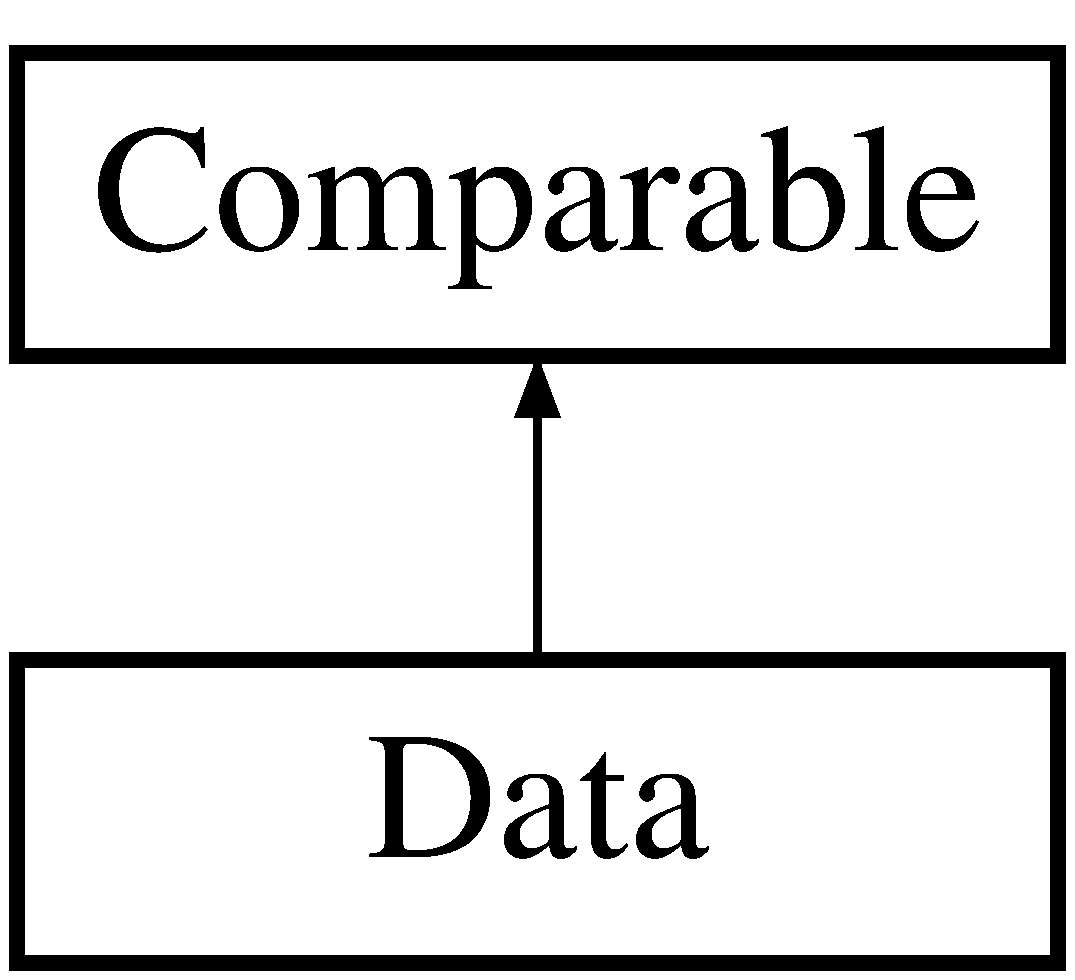
\includegraphics[height=2.000000cm]{class_data}
\end{center}
\end{figure}
\subsection*{Public Member Functions}
\begin{DoxyCompactItemize}
\item 
\hyperlink{class_data_ac9188dcb0fca3b16e8111ce3ee5c2a1c}{Data} ()
\item 
void \hyperlink{class_data_a4efe69d1a38809de935950b0c344ac94}{set\+Title} (String title)
\item 
void \hyperlink{class_data_a03a832c4735f73cf7ffd55ab0261c1aa}{set\+Year} (int year)
\item 
void \hyperlink{class_data_a7112127b737cbae7671940486a3a2f2f}{set\+Volume} (String volume)
\item 
void \hyperlink{class_data_a368b24c15d79a0ec0c33f031f489d616}{set\+Pages} (String pages)
\item 
void \hyperlink{class_data_a18f402932ef14e0f351e9419def6d840}{set\+Journal\+\_\+booktitle} (String journal\+\_\+booktitle)
\item 
void \hyperlink{class_data_aee77b766926cff5acb486c8993c39607}{add\+Author} (String \+\_\+author)
\item 
void \hyperlink{class_data_a0f3fd3bbb22e15759be23fc1bf8a54b9}{add\+Url} (String \+\_\+url)
\item 
String \hyperlink{class_data_a4163034911e6f4b0b3e4bd2135824c5f}{get\+Author} ()
\item 
String \hyperlink{class_data_ae19e8172a648699e26eceab342383e4d}{get\+Url} ()
\item 
String \hyperlink{class_data_abed831f7e25a9173f7120dbf9bbac2bd}{get\+Title} ()
\item 
int \hyperlink{class_data_afd9f8a0a7ddf04b40ac2c6a038f61e68}{get\+Year} ()
\item 
String \hyperlink{class_data_a57d3cdf8d58ca9761c9c1873a352ad9e}{get\+Volume} ()
\item 
String \hyperlink{class_data_a7c34cb99f132d8fb526462d59a033aa8}{get\+Pages} ()
\item 
String \hyperlink{class_data_ac1e4612845513c0826716962bcad943c}{get\+Journal\+\_\+booktitle} ()
\item 
Array\+List$<$ String $>$ \hyperlink{class_data_a3e01a97f8e6695e9ae4bbdfb4e012127}{get\+Raw\+Author} ()
\item 
int \hyperlink{class_data_af0585a116e5d386a0d513b8f1549411a}{compare\+To} (Object o)
\item 
String \hyperlink{class_data_a7c190e5a2f3f11629a13a90d05e9e1cf}{to\+String} ()
\end{DoxyCompactItemize}


\subsection{Constructor \& Destructor Documentation}
\hypertarget{class_data_ac9188dcb0fca3b16e8111ce3ee5c2a1c}{}\label{class_data_ac9188dcb0fca3b16e8111ce3ee5c2a1c} 
\index{Data@{Data}!Data@{Data}}
\index{Data@{Data}!Data@{Data}}
\subsubsection{\texorpdfstring{Data()}{Data()}}
{\footnotesize\ttfamily Data.\+Data (\begin{DoxyParamCaption}{ }\end{DoxyParamCaption})}



\subsection{Member Function Documentation}
\hypertarget{class_data_aee77b766926cff5acb486c8993c39607}{}\label{class_data_aee77b766926cff5acb486c8993c39607} 
\index{Data@{Data}!add\+Author@{add\+Author}}
\index{add\+Author@{add\+Author}!Data@{Data}}
\subsubsection{\texorpdfstring{add\+Author()}{addAuthor()}}
{\footnotesize\ttfamily void Data.\+add\+Author (\begin{DoxyParamCaption}\item[{String}]{\+\_\+author }\end{DoxyParamCaption})}

\hypertarget{class_data_a0f3fd3bbb22e15759be23fc1bf8a54b9}{}\label{class_data_a0f3fd3bbb22e15759be23fc1bf8a54b9} 
\index{Data@{Data}!add\+Url@{add\+Url}}
\index{add\+Url@{add\+Url}!Data@{Data}}
\subsubsection{\texorpdfstring{add\+Url()}{addUrl()}}
{\footnotesize\ttfamily void Data.\+add\+Url (\begin{DoxyParamCaption}\item[{String}]{\+\_\+url }\end{DoxyParamCaption})}

\hypertarget{class_data_af0585a116e5d386a0d513b8f1549411a}{}\label{class_data_af0585a116e5d386a0d513b8f1549411a} 
\index{Data@{Data}!compare\+To@{compare\+To}}
\index{compare\+To@{compare\+To}!Data@{Data}}
\subsubsection{\texorpdfstring{compare\+To()}{compareTo()}}
{\footnotesize\ttfamily int Data.\+compare\+To (\begin{DoxyParamCaption}\item[{Object}]{o }\end{DoxyParamCaption})}

\hypertarget{class_data_a4163034911e6f4b0b3e4bd2135824c5f}{}\label{class_data_a4163034911e6f4b0b3e4bd2135824c5f} 
\index{Data@{Data}!get\+Author@{get\+Author}}
\index{get\+Author@{get\+Author}!Data@{Data}}
\subsubsection{\texorpdfstring{get\+Author()}{getAuthor()}}
{\footnotesize\ttfamily String Data.\+get\+Author (\begin{DoxyParamCaption}{ }\end{DoxyParamCaption})}

\hypertarget{class_data_ac1e4612845513c0826716962bcad943c}{}\label{class_data_ac1e4612845513c0826716962bcad943c} 
\index{Data@{Data}!get\+Journal\+\_\+booktitle@{get\+Journal\+\_\+booktitle}}
\index{get\+Journal\+\_\+booktitle@{get\+Journal\+\_\+booktitle}!Data@{Data}}
\subsubsection{\texorpdfstring{get\+Journal\+\_\+booktitle()}{getJournal\_booktitle()}}
{\footnotesize\ttfamily String Data.\+get\+Journal\+\_\+booktitle (\begin{DoxyParamCaption}{ }\end{DoxyParamCaption})}

\hypertarget{class_data_a7c34cb99f132d8fb526462d59a033aa8}{}\label{class_data_a7c34cb99f132d8fb526462d59a033aa8} 
\index{Data@{Data}!get\+Pages@{get\+Pages}}
\index{get\+Pages@{get\+Pages}!Data@{Data}}
\subsubsection{\texorpdfstring{get\+Pages()}{getPages()}}
{\footnotesize\ttfamily String Data.\+get\+Pages (\begin{DoxyParamCaption}{ }\end{DoxyParamCaption})}

\hypertarget{class_data_a3e01a97f8e6695e9ae4bbdfb4e012127}{}\label{class_data_a3e01a97f8e6695e9ae4bbdfb4e012127} 
\index{Data@{Data}!get\+Raw\+Author@{get\+Raw\+Author}}
\index{get\+Raw\+Author@{get\+Raw\+Author}!Data@{Data}}
\subsubsection{\texorpdfstring{get\+Raw\+Author()}{getRawAuthor()}}
{\footnotesize\ttfamily Array\+List$<$String$>$ Data.\+get\+Raw\+Author (\begin{DoxyParamCaption}{ }\end{DoxyParamCaption})}

\hypertarget{class_data_abed831f7e25a9173f7120dbf9bbac2bd}{}\label{class_data_abed831f7e25a9173f7120dbf9bbac2bd} 
\index{Data@{Data}!get\+Title@{get\+Title}}
\index{get\+Title@{get\+Title}!Data@{Data}}
\subsubsection{\texorpdfstring{get\+Title()}{getTitle()}}
{\footnotesize\ttfamily String Data.\+get\+Title (\begin{DoxyParamCaption}{ }\end{DoxyParamCaption})}

\hypertarget{class_data_ae19e8172a648699e26eceab342383e4d}{}\label{class_data_ae19e8172a648699e26eceab342383e4d} 
\index{Data@{Data}!get\+Url@{get\+Url}}
\index{get\+Url@{get\+Url}!Data@{Data}}
\subsubsection{\texorpdfstring{get\+Url()}{getUrl()}}
{\footnotesize\ttfamily String Data.\+get\+Url (\begin{DoxyParamCaption}{ }\end{DoxyParamCaption})}

\hypertarget{class_data_a57d3cdf8d58ca9761c9c1873a352ad9e}{}\label{class_data_a57d3cdf8d58ca9761c9c1873a352ad9e} 
\index{Data@{Data}!get\+Volume@{get\+Volume}}
\index{get\+Volume@{get\+Volume}!Data@{Data}}
\subsubsection{\texorpdfstring{get\+Volume()}{getVolume()}}
{\footnotesize\ttfamily String Data.\+get\+Volume (\begin{DoxyParamCaption}{ }\end{DoxyParamCaption})}

\hypertarget{class_data_afd9f8a0a7ddf04b40ac2c6a038f61e68}{}\label{class_data_afd9f8a0a7ddf04b40ac2c6a038f61e68} 
\index{Data@{Data}!get\+Year@{get\+Year}}
\index{get\+Year@{get\+Year}!Data@{Data}}
\subsubsection{\texorpdfstring{get\+Year()}{getYear()}}
{\footnotesize\ttfamily int Data.\+get\+Year (\begin{DoxyParamCaption}{ }\end{DoxyParamCaption})}

\hypertarget{class_data_a18f402932ef14e0f351e9419def6d840}{}\label{class_data_a18f402932ef14e0f351e9419def6d840} 
\index{Data@{Data}!set\+Journal\+\_\+booktitle@{set\+Journal\+\_\+booktitle}}
\index{set\+Journal\+\_\+booktitle@{set\+Journal\+\_\+booktitle}!Data@{Data}}
\subsubsection{\texorpdfstring{set\+Journal\+\_\+booktitle()}{setJournal\_booktitle()}}
{\footnotesize\ttfamily void Data.\+set\+Journal\+\_\+booktitle (\begin{DoxyParamCaption}\item[{String}]{journal\+\_\+booktitle }\end{DoxyParamCaption})}

\hypertarget{class_data_a368b24c15d79a0ec0c33f031f489d616}{}\label{class_data_a368b24c15d79a0ec0c33f031f489d616} 
\index{Data@{Data}!set\+Pages@{set\+Pages}}
\index{set\+Pages@{set\+Pages}!Data@{Data}}
\subsubsection{\texorpdfstring{set\+Pages()}{setPages()}}
{\footnotesize\ttfamily void Data.\+set\+Pages (\begin{DoxyParamCaption}\item[{String}]{pages }\end{DoxyParamCaption})}

\hypertarget{class_data_a4efe69d1a38809de935950b0c344ac94}{}\label{class_data_a4efe69d1a38809de935950b0c344ac94} 
\index{Data@{Data}!set\+Title@{set\+Title}}
\index{set\+Title@{set\+Title}!Data@{Data}}
\subsubsection{\texorpdfstring{set\+Title()}{setTitle()}}
{\footnotesize\ttfamily void Data.\+set\+Title (\begin{DoxyParamCaption}\item[{String}]{title }\end{DoxyParamCaption})}

\hypertarget{class_data_a7112127b737cbae7671940486a3a2f2f}{}\label{class_data_a7112127b737cbae7671940486a3a2f2f} 
\index{Data@{Data}!set\+Volume@{set\+Volume}}
\index{set\+Volume@{set\+Volume}!Data@{Data}}
\subsubsection{\texorpdfstring{set\+Volume()}{setVolume()}}
{\footnotesize\ttfamily void Data.\+set\+Volume (\begin{DoxyParamCaption}\item[{String}]{volume }\end{DoxyParamCaption})}

\hypertarget{class_data_a03a832c4735f73cf7ffd55ab0261c1aa}{}\label{class_data_a03a832c4735f73cf7ffd55ab0261c1aa} 
\index{Data@{Data}!set\+Year@{set\+Year}}
\index{set\+Year@{set\+Year}!Data@{Data}}
\subsubsection{\texorpdfstring{set\+Year()}{setYear()}}
{\footnotesize\ttfamily void Data.\+set\+Year (\begin{DoxyParamCaption}\item[{int}]{year }\end{DoxyParamCaption})}

\hypertarget{class_data_a7c190e5a2f3f11629a13a90d05e9e1cf}{}\label{class_data_a7c190e5a2f3f11629a13a90d05e9e1cf} 
\index{Data@{Data}!to\+String@{to\+String}}
\index{to\+String@{to\+String}!Data@{Data}}
\subsubsection{\texorpdfstring{to\+String()}{toString()}}
{\footnotesize\ttfamily String Data.\+to\+String (\begin{DoxyParamCaption}{ }\end{DoxyParamCaption})}



The documentation for this class was generated from the following file\+:\begin{DoxyCompactItemize}
\item 
\hyperlink{_data_8java}{Data.\+java}\end{DoxyCompactItemize}

\hypertarget{class_database}{}\section{Database Class Reference}
\label{class_database}\index{Database@{Database}}
\subsection*{Static Public Attributes}
\begin{DoxyCompactItemize}
\item 
static Array\+List$<$ \hyperlink{class_data}{Data} $>$ \hyperlink{class_database_a3452b90eeadc0c854bd314663a599dde}{all\+Data} = new Array\+List$<$$>$()
\end{DoxyCompactItemize}


\subsection{Member Data Documentation}
\hypertarget{class_database_a3452b90eeadc0c854bd314663a599dde}{}\label{class_database_a3452b90eeadc0c854bd314663a599dde} 
\index{Database@{Database}!all\+Data@{all\+Data}}
\index{all\+Data@{all\+Data}!Database@{Database}}
\subsubsection{\texorpdfstring{all\+Data}{allData}}
{\footnotesize\ttfamily Array\+List$<$\hyperlink{class_data}{Data}$>$ Database.\+all\+Data = new Array\+List$<$$>$()\hspace{0.3cm}{\ttfamily [static]}}



The documentation for this class was generated from the following file\+:\begin{DoxyCompactItemize}
\item 
src/\hyperlink{_database_8java}{Database.\+java}\end{DoxyCompactItemize}

\hypertarget{classmain_class}{}\section{main\+Class Class Reference}
\label{classmain_class}\index{main\+Class@{main\+Class}}
\subsection*{Static Public Member Functions}
\begin{DoxyCompactItemize}
\item 
static void \hyperlink{classmain_class_a0b4ecc5e71b50c684de72b0b691a14d0}{main} (String\mbox{[}$\,$\mbox{]} args)
\end{DoxyCompactItemize}


\subsection{Member Function Documentation}
\hypertarget{classmain_class_a0b4ecc5e71b50c684de72b0b691a14d0}{}\label{classmain_class_a0b4ecc5e71b50c684de72b0b691a14d0} 
\index{main\+Class@{main\+Class}!main@{main}}
\index{main@{main}!main\+Class@{main\+Class}}
\subsubsection{\texorpdfstring{main()}{main()}}
{\footnotesize\ttfamily static void main\+Class.\+main (\begin{DoxyParamCaption}\item[{String \mbox{[}$\,$\mbox{]}}]{args }\end{DoxyParamCaption})\hspace{0.3cm}{\ttfamily [static]}}



The documentation for this class was generated from the following file\+:\begin{DoxyCompactItemize}
\item 
\hyperlink{main_class_8java}{main\+Class.\+java}\end{DoxyCompactItemize}

\hypertarget{classmy_frame}{}\section{my\+Frame Class Reference}
\label{classmy_frame}\index{my\+Frame@{my\+Frame}}
Inheritance diagram for my\+Frame\+:\begin{figure}[H]
\begin{center}
\leavevmode
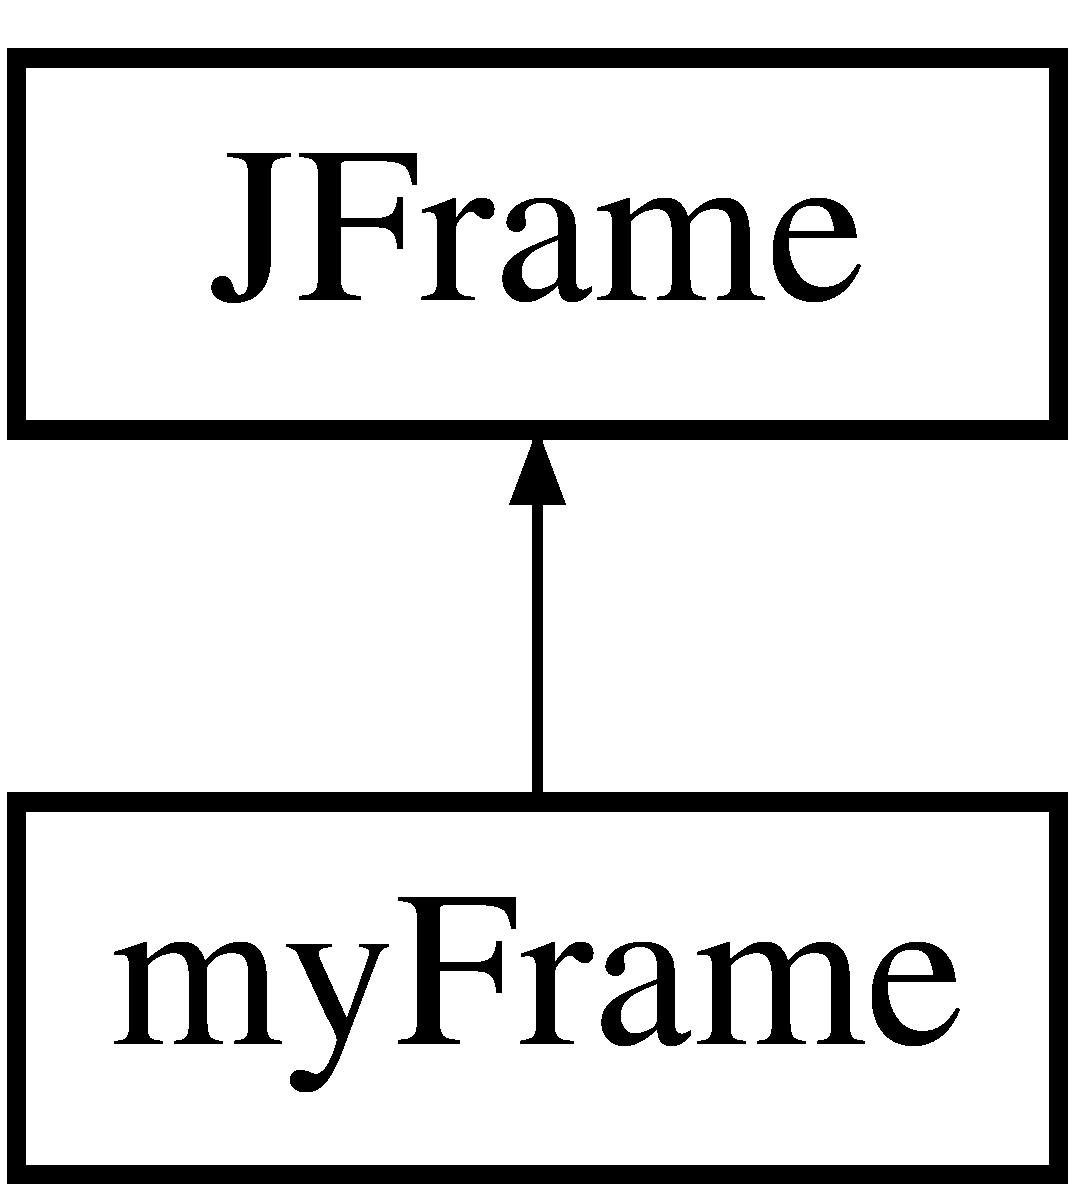
\includegraphics[height=2.000000cm]{classmy_frame}
\end{center}
\end{figure}
\subsection*{Public Member Functions}
\begin{DoxyCompactItemize}
\item 
\hyperlink{classmy_frame_a2b3c0cea5de20595de9c29760f8b69f3}{my\+Frame} (\hyperlink{classmy_panel}{my\+Panel} panel)
\end{DoxyCompactItemize}
\subsection*{Static Public Member Functions}
\begin{DoxyCompactItemize}
\item 
static J\+Progress\+Bar \hyperlink{classmy_frame_ab4821a86dfc373a36ef2d654cf81f238}{get\+Bar} ()
\end{DoxyCompactItemize}


\subsection{Constructor \& Destructor Documentation}
\hypertarget{classmy_frame_a2b3c0cea5de20595de9c29760f8b69f3}{}\label{classmy_frame_a2b3c0cea5de20595de9c29760f8b69f3} 
\index{my\+Frame@{my\+Frame}!my\+Frame@{my\+Frame}}
\index{my\+Frame@{my\+Frame}!my\+Frame@{my\+Frame}}
\subsubsection{\texorpdfstring{my\+Frame()}{myFrame()}}
{\footnotesize\ttfamily my\+Frame.\+my\+Frame (\begin{DoxyParamCaption}\item[{\hyperlink{classmy_panel}{my\+Panel}}]{panel }\end{DoxyParamCaption})}



\subsection{Member Function Documentation}
\hypertarget{classmy_frame_ab4821a86dfc373a36ef2d654cf81f238}{}\label{classmy_frame_ab4821a86dfc373a36ef2d654cf81f238} 
\index{my\+Frame@{my\+Frame}!get\+Bar@{get\+Bar}}
\index{get\+Bar@{get\+Bar}!my\+Frame@{my\+Frame}}
\subsubsection{\texorpdfstring{get\+Bar()}{getBar()}}
{\footnotesize\ttfamily static J\+Progress\+Bar my\+Frame.\+get\+Bar (\begin{DoxyParamCaption}{ }\end{DoxyParamCaption})\hspace{0.3cm}{\ttfamily [static]}}



The documentation for this class was generated from the following file\+:\begin{DoxyCompactItemize}
\item 
\hyperlink{my_frame_8java}{my\+Frame.\+java}\end{DoxyCompactItemize}

\hypertarget{classmy_panel}{}\section{my\+Panel Class Reference}
\label{classmy_panel}\index{my\+Panel@{my\+Panel}}
\subsection*{Public Member Functions}
\begin{DoxyCompactItemize}
\item 
\hyperlink{classmy_panel_ab3caf63718b52c0f771983dc83b2d950}{my\+Panel} ()
\item 
void \hyperlink{classmy_panel_ac67bebd824b15236aa5213673cd49c88}{working\+Of\+Buttons} ()
\item 
J\+Panel \hyperlink{classmy_panel_a259592e52478c99ae70c9e962ad17236}{get\+Panel} ()
\end{DoxyCompactItemize}


\subsection{Constructor \& Destructor Documentation}
\hypertarget{classmy_panel_ab3caf63718b52c0f771983dc83b2d950}{}\label{classmy_panel_ab3caf63718b52c0f771983dc83b2d950} 
\index{my\+Panel@{my\+Panel}!my\+Panel@{my\+Panel}}
\index{my\+Panel@{my\+Panel}!my\+Panel@{my\+Panel}}
\subsubsection{\texorpdfstring{my\+Panel()}{myPanel()}}
{\footnotesize\ttfamily my\+Panel.\+my\+Panel (\begin{DoxyParamCaption}{ }\end{DoxyParamCaption})}



\subsection{Member Function Documentation}
\hypertarget{classmy_panel_a259592e52478c99ae70c9e962ad17236}{}\label{classmy_panel_a259592e52478c99ae70c9e962ad17236} 
\index{my\+Panel@{my\+Panel}!get\+Panel@{get\+Panel}}
\index{get\+Panel@{get\+Panel}!my\+Panel@{my\+Panel}}
\subsubsection{\texorpdfstring{get\+Panel()}{getPanel()}}
{\footnotesize\ttfamily J\+Panel my\+Panel.\+get\+Panel (\begin{DoxyParamCaption}{ }\end{DoxyParamCaption})}

\hypertarget{classmy_panel_ac67bebd824b15236aa5213673cd49c88}{}\label{classmy_panel_ac67bebd824b15236aa5213673cd49c88} 
\index{my\+Panel@{my\+Panel}!working\+Of\+Buttons@{working\+Of\+Buttons}}
\index{working\+Of\+Buttons@{working\+Of\+Buttons}!my\+Panel@{my\+Panel}}
\subsubsection{\texorpdfstring{working\+Of\+Buttons()}{workingOfButtons()}}
{\footnotesize\ttfamily void my\+Panel.\+working\+Of\+Buttons (\begin{DoxyParamCaption}{ }\end{DoxyParamCaption})}



The documentation for this class was generated from the following file\+:\begin{DoxyCompactItemize}
\item 
\hyperlink{my_panel_8java}{my\+Panel.\+java}\end{DoxyCompactItemize}

\hypertarget{classmy_query1_panel}{}\section{my\+Query1\+Panel Class Reference}
\label{classmy_query1_panel}\index{my\+Query1\+Panel@{my\+Query1\+Panel}}
\subsection*{Public Member Functions}
\begin{DoxyCompactItemize}
\item 
\hyperlink{classmy_query1_panel_add6c4e09fbce53ae0b2eb34e2da0c55e}{my\+Query1\+Panel} ()
\item 
void \hyperlink{classmy_query1_panel_a0a640aa15c5356a9eab718201267a245}{prepare\+Buttons} ()
\end{DoxyCompactItemize}
\subsection*{Protected Attributes}
\begin{DoxyCompactItemize}
\item 
J\+Panel \hyperlink{classmy_query1_panel_aba2fe28e793bc84fe789e98c7b89e065}{panel2} =new J\+Panel(new Grid\+Bag\+Layout())
\item 
J\+Button \hyperlink{classmy_query1_panel_a0e0a620150837e7d0caa3386fdd1879b}{reset\+Button}
\item 
J\+Text\+Field \hyperlink{classmy_query1_panel_a60b95255f8c6ffeb063ca97c79206c49}{since\+Year\+Text\+Field}
\item 
J\+Combo\+Box \hyperlink{classmy_query1_panel_ac662f986c33598e85559ac3d93f634b0}{year\+Combo}
\item 
Checkbox \hyperlink{classmy_query1_panel_a112a1c15d47ccd9a16a3d5d4e7211809}{chk\+Sort\+By\+Year}
\item 
Checkbox\+Group \hyperlink{classmy_query1_panel_a5ae5e5e6cfc109b6a15ac6811604a5c1}{sort}
\end{DoxyCompactItemize}
\subsection*{Private Member Functions}
\begin{DoxyCompactItemize}
\item 
void \hyperlink{classmy_query1_panel_ab03012b238b9d2e22928784002a28e7f}{colorize} ()
\item 
void \hyperlink{classmy_query1_panel_ad7b5f2e116e6e88a6d8c71f2c0633b42}{prepare\+Check\+Box\+UI} ()
\item 
void \hyperlink{classmy_query1_panel_a31942385ff8324fbe1220229037b2cf6}{prepare\+Year\+Search\+Combo\+Box} ()
\item 
void \hyperlink{classmy_query1_panel_a1d028e5e8a80ea2a14956e7facfe3ce3}{Year\+Search\+UI} ()
\item 
void \hyperlink{classmy_query1_panel_ab15b9ca3d19fe07f6c660231ba97cd47}{prepare\+Search\+By\+Combo\+Box} ()
\end{DoxyCompactItemize}
\subsection*{Private Attributes}
\begin{DoxyCompactItemize}
\item 
Grid\+Bag\+Constraints \hyperlink{classmy_query1_panel_a950bb4c948bbc32c52dcd51b9c37a8fd}{panel2gbc} = new Grid\+Bag\+Constraints()
\item 
J\+Label \hyperlink{classmy_query1_panel_a4a96735d4624a707ca5c9f774a95f054}{since\+Year}
\end{DoxyCompactItemize}


\subsection{Constructor \& Destructor Documentation}
\hypertarget{classmy_query1_panel_add6c4e09fbce53ae0b2eb34e2da0c55e}{}\label{classmy_query1_panel_add6c4e09fbce53ae0b2eb34e2da0c55e} 
\index{my\+Query1\+Panel@{my\+Query1\+Panel}!my\+Query1\+Panel@{my\+Query1\+Panel}}
\index{my\+Query1\+Panel@{my\+Query1\+Panel}!my\+Query1\+Panel@{my\+Query1\+Panel}}
\subsubsection{\texorpdfstring{my\+Query1\+Panel()}{myQuery1Panel()}}
{\footnotesize\ttfamily my\+Query1\+Panel.\+my\+Query1\+Panel (\begin{DoxyParamCaption}{ }\end{DoxyParamCaption})}



\subsection{Member Function Documentation}
\hypertarget{classmy_query1_panel_ab03012b238b9d2e22928784002a28e7f}{}\label{classmy_query1_panel_ab03012b238b9d2e22928784002a28e7f} 
\index{my\+Query1\+Panel@{my\+Query1\+Panel}!colorize@{colorize}}
\index{colorize@{colorize}!my\+Query1\+Panel@{my\+Query1\+Panel}}
\subsubsection{\texorpdfstring{colorize()}{colorize()}}
{\footnotesize\ttfamily void my\+Query1\+Panel.\+colorize (\begin{DoxyParamCaption}{ }\end{DoxyParamCaption})\hspace{0.3cm}{\ttfamily [private]}}

\hypertarget{classmy_query1_panel_a0a640aa15c5356a9eab718201267a245}{}\label{classmy_query1_panel_a0a640aa15c5356a9eab718201267a245} 
\index{my\+Query1\+Panel@{my\+Query1\+Panel}!prepare\+Buttons@{prepare\+Buttons}}
\index{prepare\+Buttons@{prepare\+Buttons}!my\+Query1\+Panel@{my\+Query1\+Panel}}
\subsubsection{\texorpdfstring{prepare\+Buttons()}{prepareButtons()}}
{\footnotesize\ttfamily void my\+Query1\+Panel.\+prepare\+Buttons (\begin{DoxyParamCaption}{ }\end{DoxyParamCaption})}

\hypertarget{classmy_query1_panel_ad7b5f2e116e6e88a6d8c71f2c0633b42}{}\label{classmy_query1_panel_ad7b5f2e116e6e88a6d8c71f2c0633b42} 
\index{my\+Query1\+Panel@{my\+Query1\+Panel}!prepare\+Check\+Box\+UI@{prepare\+Check\+Box\+UI}}
\index{prepare\+Check\+Box\+UI@{prepare\+Check\+Box\+UI}!my\+Query1\+Panel@{my\+Query1\+Panel}}
\subsubsection{\texorpdfstring{prepare\+Check\+Box\+U\+I()}{prepareCheckBoxUI()}}
{\footnotesize\ttfamily void my\+Query1\+Panel.\+prepare\+Check\+Box\+UI (\begin{DoxyParamCaption}{ }\end{DoxyParamCaption})\hspace{0.3cm}{\ttfamily [private]}}

\hypertarget{classmy_query1_panel_ab15b9ca3d19fe07f6c660231ba97cd47}{}\label{classmy_query1_panel_ab15b9ca3d19fe07f6c660231ba97cd47} 
\index{my\+Query1\+Panel@{my\+Query1\+Panel}!prepare\+Search\+By\+Combo\+Box@{prepare\+Search\+By\+Combo\+Box}}
\index{prepare\+Search\+By\+Combo\+Box@{prepare\+Search\+By\+Combo\+Box}!my\+Query1\+Panel@{my\+Query1\+Panel}}
\subsubsection{\texorpdfstring{prepare\+Search\+By\+Combo\+Box()}{prepareSearchByComboBox()}}
{\footnotesize\ttfamily void my\+Query1\+Panel.\+prepare\+Search\+By\+Combo\+Box (\begin{DoxyParamCaption}{ }\end{DoxyParamCaption})\hspace{0.3cm}{\ttfamily [private]}}

\hypertarget{classmy_query1_panel_a31942385ff8324fbe1220229037b2cf6}{}\label{classmy_query1_panel_a31942385ff8324fbe1220229037b2cf6} 
\index{my\+Query1\+Panel@{my\+Query1\+Panel}!prepare\+Year\+Search\+Combo\+Box@{prepare\+Year\+Search\+Combo\+Box}}
\index{prepare\+Year\+Search\+Combo\+Box@{prepare\+Year\+Search\+Combo\+Box}!my\+Query1\+Panel@{my\+Query1\+Panel}}
\subsubsection{\texorpdfstring{prepare\+Year\+Search\+Combo\+Box()}{prepareYearSearchComboBox()}}
{\footnotesize\ttfamily void my\+Query1\+Panel.\+prepare\+Year\+Search\+Combo\+Box (\begin{DoxyParamCaption}{ }\end{DoxyParamCaption})\hspace{0.3cm}{\ttfamily [private]}}

\hypertarget{classmy_query1_panel_a1d028e5e8a80ea2a14956e7facfe3ce3}{}\label{classmy_query1_panel_a1d028e5e8a80ea2a14956e7facfe3ce3} 
\index{my\+Query1\+Panel@{my\+Query1\+Panel}!Year\+Search\+UI@{Year\+Search\+UI}}
\index{Year\+Search\+UI@{Year\+Search\+UI}!my\+Query1\+Panel@{my\+Query1\+Panel}}
\subsubsection{\texorpdfstring{Year\+Search\+U\+I()}{YearSearchUI()}}
{\footnotesize\ttfamily void my\+Query1\+Panel.\+Year\+Search\+UI (\begin{DoxyParamCaption}{ }\end{DoxyParamCaption})\hspace{0.3cm}{\ttfamily [private]}}



\subsection{Member Data Documentation}
\hypertarget{classmy_query1_panel_a112a1c15d47ccd9a16a3d5d4e7211809}{}\label{classmy_query1_panel_a112a1c15d47ccd9a16a3d5d4e7211809} 
\index{my\+Query1\+Panel@{my\+Query1\+Panel}!chk\+Sort\+By\+Year@{chk\+Sort\+By\+Year}}
\index{chk\+Sort\+By\+Year@{chk\+Sort\+By\+Year}!my\+Query1\+Panel@{my\+Query1\+Panel}}
\subsubsection{\texorpdfstring{chk\+Sort\+By\+Year}{chkSortByYear}}
{\footnotesize\ttfamily Checkbox my\+Query1\+Panel.\+chk\+Sort\+By\+Year\hspace{0.3cm}{\ttfamily [protected]}}

\hypertarget{classmy_query1_panel_aba2fe28e793bc84fe789e98c7b89e065}{}\label{classmy_query1_panel_aba2fe28e793bc84fe789e98c7b89e065} 
\index{my\+Query1\+Panel@{my\+Query1\+Panel}!panel2@{panel2}}
\index{panel2@{panel2}!my\+Query1\+Panel@{my\+Query1\+Panel}}
\subsubsection{\texorpdfstring{panel2}{panel2}}
{\footnotesize\ttfamily J\+Panel my\+Query1\+Panel.\+panel2 =new J\+Panel(new Grid\+Bag\+Layout())\hspace{0.3cm}{\ttfamily [protected]}}

\hypertarget{classmy_query1_panel_a950bb4c948bbc32c52dcd51b9c37a8fd}{}\label{classmy_query1_panel_a950bb4c948bbc32c52dcd51b9c37a8fd} 
\index{my\+Query1\+Panel@{my\+Query1\+Panel}!panel2gbc@{panel2gbc}}
\index{panel2gbc@{panel2gbc}!my\+Query1\+Panel@{my\+Query1\+Panel}}
\subsubsection{\texorpdfstring{panel2gbc}{panel2gbc}}
{\footnotesize\ttfamily Grid\+Bag\+Constraints my\+Query1\+Panel.\+panel2gbc = new Grid\+Bag\+Constraints()\hspace{0.3cm}{\ttfamily [private]}}

\hypertarget{classmy_query1_panel_a0e0a620150837e7d0caa3386fdd1879b}{}\label{classmy_query1_panel_a0e0a620150837e7d0caa3386fdd1879b} 
\index{my\+Query1\+Panel@{my\+Query1\+Panel}!reset\+Button@{reset\+Button}}
\index{reset\+Button@{reset\+Button}!my\+Query1\+Panel@{my\+Query1\+Panel}}
\subsubsection{\texorpdfstring{reset\+Button}{resetButton}}
{\footnotesize\ttfamily J\+Button my\+Query1\+Panel.\+reset\+Button\hspace{0.3cm}{\ttfamily [protected]}}

\hypertarget{classmy_query1_panel_a4a96735d4624a707ca5c9f774a95f054}{}\label{classmy_query1_panel_a4a96735d4624a707ca5c9f774a95f054} 
\index{my\+Query1\+Panel@{my\+Query1\+Panel}!since\+Year@{since\+Year}}
\index{since\+Year@{since\+Year}!my\+Query1\+Panel@{my\+Query1\+Panel}}
\subsubsection{\texorpdfstring{since\+Year}{sinceYear}}
{\footnotesize\ttfamily J\+Label my\+Query1\+Panel.\+since\+Year\hspace{0.3cm}{\ttfamily [private]}}

\hypertarget{classmy_query1_panel_a60b95255f8c6ffeb063ca97c79206c49}{}\label{classmy_query1_panel_a60b95255f8c6ffeb063ca97c79206c49} 
\index{my\+Query1\+Panel@{my\+Query1\+Panel}!since\+Year\+Text\+Field@{since\+Year\+Text\+Field}}
\index{since\+Year\+Text\+Field@{since\+Year\+Text\+Field}!my\+Query1\+Panel@{my\+Query1\+Panel}}
\subsubsection{\texorpdfstring{since\+Year\+Text\+Field}{sinceYearTextField}}
{\footnotesize\ttfamily J\+Text\+Field my\+Query1\+Panel.\+since\+Year\+Text\+Field\hspace{0.3cm}{\ttfamily [protected]}}

\hypertarget{classmy_query1_panel_a5ae5e5e6cfc109b6a15ac6811604a5c1}{}\label{classmy_query1_panel_a5ae5e5e6cfc109b6a15ac6811604a5c1} 
\index{my\+Query1\+Panel@{my\+Query1\+Panel}!sort@{sort}}
\index{sort@{sort}!my\+Query1\+Panel@{my\+Query1\+Panel}}
\subsubsection{\texorpdfstring{sort}{sort}}
{\footnotesize\ttfamily Checkbox\+Group my\+Query1\+Panel.\+sort\hspace{0.3cm}{\ttfamily [protected]}}

\hypertarget{classmy_query1_panel_ac662f986c33598e85559ac3d93f634b0}{}\label{classmy_query1_panel_ac662f986c33598e85559ac3d93f634b0} 
\index{my\+Query1\+Panel@{my\+Query1\+Panel}!year\+Combo@{year\+Combo}}
\index{year\+Combo@{year\+Combo}!my\+Query1\+Panel@{my\+Query1\+Panel}}
\subsubsection{\texorpdfstring{year\+Combo}{yearCombo}}
{\footnotesize\ttfamily J\+Combo\+Box my\+Query1\+Panel.\+year\+Combo\hspace{0.3cm}{\ttfamily [protected]}}



The documentation for this class was generated from the following file\+:\begin{DoxyCompactItemize}
\item 
src/\hyperlink{my_query1_panel_8java}{my\+Query1\+Panel.\+java}\end{DoxyCompactItemize}

\hypertarget{classmy_query2_panel}{}\section{my\+Query2\+Panel Class Reference}
\label{classmy_query2_panel}\index{my\+Query2\+Panel@{my\+Query2\+Panel}}
\subsection*{Public Member Functions}
\begin{DoxyCompactItemize}
\item 
\hyperlink{classmy_query2_panel_a6bc36043976b346eb7e46eea21956042}{my\+Query2\+Panel} ()
\item 
void \hyperlink{classmy_query2_panel_a734aedb77732969bf2c9834104a0d59e}{prepare\+Gui} ()
\item 
void \hyperlink{classmy_query2_panel_a7ff73944523f85b4c3a79a4c019f73d3}{button\+Working} ()
\item 
J\+Panel \hyperlink{classmy_query2_panel_a7977bb42f9d5959684f805e08337d27b}{get\+Panel} ()
\end{DoxyCompactItemize}


\subsection{Constructor \& Destructor Documentation}
\hypertarget{classmy_query2_panel_a6bc36043976b346eb7e46eea21956042}{}\label{classmy_query2_panel_a6bc36043976b346eb7e46eea21956042} 
\index{my\+Query2\+Panel@{my\+Query2\+Panel}!my\+Query2\+Panel@{my\+Query2\+Panel}}
\index{my\+Query2\+Panel@{my\+Query2\+Panel}!my\+Query2\+Panel@{my\+Query2\+Panel}}
\subsubsection{\texorpdfstring{my\+Query2\+Panel()}{myQuery2Panel()}}
{\footnotesize\ttfamily my\+Query2\+Panel.\+my\+Query2\+Panel (\begin{DoxyParamCaption}{ }\end{DoxyParamCaption})}



\subsection{Member Function Documentation}
\hypertarget{classmy_query2_panel_a7ff73944523f85b4c3a79a4c019f73d3}{}\label{classmy_query2_panel_a7ff73944523f85b4c3a79a4c019f73d3} 
\index{my\+Query2\+Panel@{my\+Query2\+Panel}!button\+Working@{button\+Working}}
\index{button\+Working@{button\+Working}!my\+Query2\+Panel@{my\+Query2\+Panel}}
\subsubsection{\texorpdfstring{button\+Working()}{buttonWorking()}}
{\footnotesize\ttfamily void my\+Query2\+Panel.\+button\+Working (\begin{DoxyParamCaption}{ }\end{DoxyParamCaption})}

\hypertarget{classmy_query2_panel_a7977bb42f9d5959684f805e08337d27b}{}\label{classmy_query2_panel_a7977bb42f9d5959684f805e08337d27b} 
\index{my\+Query2\+Panel@{my\+Query2\+Panel}!get\+Panel@{get\+Panel}}
\index{get\+Panel@{get\+Panel}!my\+Query2\+Panel@{my\+Query2\+Panel}}
\subsubsection{\texorpdfstring{get\+Panel()}{getPanel()}}
{\footnotesize\ttfamily J\+Panel my\+Query2\+Panel.\+get\+Panel (\begin{DoxyParamCaption}{ }\end{DoxyParamCaption})}

\hypertarget{classmy_query2_panel_a734aedb77732969bf2c9834104a0d59e}{}\label{classmy_query2_panel_a734aedb77732969bf2c9834104a0d59e} 
\index{my\+Query2\+Panel@{my\+Query2\+Panel}!prepare\+Gui@{prepare\+Gui}}
\index{prepare\+Gui@{prepare\+Gui}!my\+Query2\+Panel@{my\+Query2\+Panel}}
\subsubsection{\texorpdfstring{prepare\+Gui()}{prepareGui()}}
{\footnotesize\ttfamily void my\+Query2\+Panel.\+prepare\+Gui (\begin{DoxyParamCaption}{ }\end{DoxyParamCaption})}



The documentation for this class was generated from the following file\+:\begin{DoxyCompactItemize}
\item 
\hyperlink{my_query2_panel_8java}{my\+Query2\+Panel.\+java}\end{DoxyCompactItemize}

\hypertarget{classmy_query3_panel}{}\section{my\+Query3\+Panel Class Reference}
\label{classmy_query3_panel}\index{my\+Query3\+Panel@{my\+Query3\+Panel}}
\subsection*{Public Member Functions}
\begin{DoxyCompactItemize}
\item 
\hyperlink{classmy_query3_panel_a41792f89e40b96e00d365f08c64ede34}{my\+Query3\+Panel} ()
\item 
void \hyperlink{classmy_query3_panel_a0ba85999b328528fb1255d54f9e35adf}{prepare\+Gui} ()
\item 
void \hyperlink{classmy_query3_panel_a733fe7c07a4083484bde4cf976ef62dc}{button\+Working} ()
\item 
J\+Panel \hyperlink{classmy_query3_panel_a7e32c709687bc0e276dbfb4abc101c83}{get\+Panel} ()
\end{DoxyCompactItemize}


\subsection{Constructor \& Destructor Documentation}
\hypertarget{classmy_query3_panel_a41792f89e40b96e00d365f08c64ede34}{}\label{classmy_query3_panel_a41792f89e40b96e00d365f08c64ede34} 
\index{my\+Query3\+Panel@{my\+Query3\+Panel}!my\+Query3\+Panel@{my\+Query3\+Panel}}
\index{my\+Query3\+Panel@{my\+Query3\+Panel}!my\+Query3\+Panel@{my\+Query3\+Panel}}
\subsubsection{\texorpdfstring{my\+Query3\+Panel()}{myQuery3Panel()}}
{\footnotesize\ttfamily my\+Query3\+Panel.\+my\+Query3\+Panel (\begin{DoxyParamCaption}{ }\end{DoxyParamCaption})}



\subsection{Member Function Documentation}
\hypertarget{classmy_query3_panel_a733fe7c07a4083484bde4cf976ef62dc}{}\label{classmy_query3_panel_a733fe7c07a4083484bde4cf976ef62dc} 
\index{my\+Query3\+Panel@{my\+Query3\+Panel}!button\+Working@{button\+Working}}
\index{button\+Working@{button\+Working}!my\+Query3\+Panel@{my\+Query3\+Panel}}
\subsubsection{\texorpdfstring{button\+Working()}{buttonWorking()}}
{\footnotesize\ttfamily void my\+Query3\+Panel.\+button\+Working (\begin{DoxyParamCaption}{ }\end{DoxyParamCaption})}

\hypertarget{classmy_query3_panel_a7e32c709687bc0e276dbfb4abc101c83}{}\label{classmy_query3_panel_a7e32c709687bc0e276dbfb4abc101c83} 
\index{my\+Query3\+Panel@{my\+Query3\+Panel}!get\+Panel@{get\+Panel}}
\index{get\+Panel@{get\+Panel}!my\+Query3\+Panel@{my\+Query3\+Panel}}
\subsubsection{\texorpdfstring{get\+Panel()}{getPanel()}}
{\footnotesize\ttfamily J\+Panel my\+Query3\+Panel.\+get\+Panel (\begin{DoxyParamCaption}{ }\end{DoxyParamCaption})}

\hypertarget{classmy_query3_panel_a0ba85999b328528fb1255d54f9e35adf}{}\label{classmy_query3_panel_a0ba85999b328528fb1255d54f9e35adf} 
\index{my\+Query3\+Panel@{my\+Query3\+Panel}!prepare\+Gui@{prepare\+Gui}}
\index{prepare\+Gui@{prepare\+Gui}!my\+Query3\+Panel@{my\+Query3\+Panel}}
\subsubsection{\texorpdfstring{prepare\+Gui()}{prepareGui()}}
{\footnotesize\ttfamily void my\+Query3\+Panel.\+prepare\+Gui (\begin{DoxyParamCaption}{ }\end{DoxyParamCaption})}



The documentation for this class was generated from the following file\+:\begin{DoxyCompactItemize}
\item 
\hyperlink{my_query3_panel_8java}{my\+Query3\+Panel.\+java}\end{DoxyCompactItemize}

\hypertarget{class_parser}{}\section{Parser Class Reference}
\label{class_parser}\index{Parser@{Parser}}
Inheritance diagram for Parser\+:\begin{figure}[H]
\begin{center}
\leavevmode
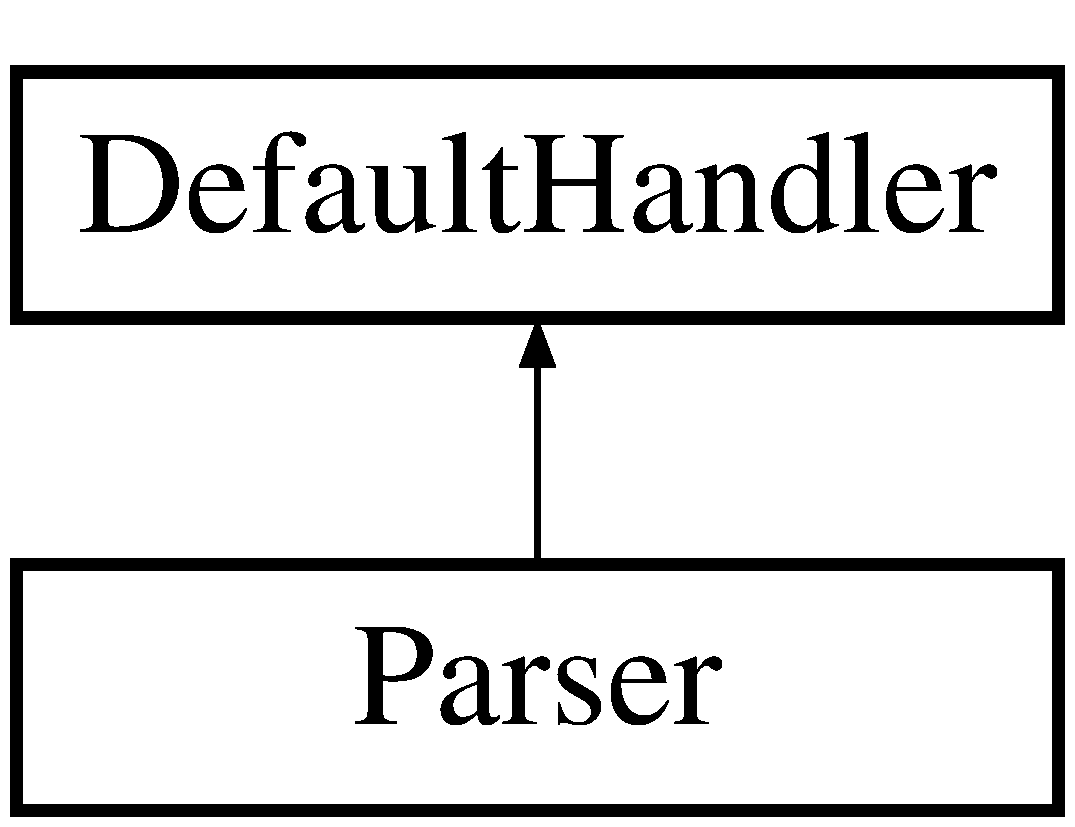
\includegraphics[height=2.000000cm]{class_parser}
\end{center}
\end{figure}
\subsection*{Classes}
\begin{DoxyCompactItemize}
\item 
class {\bfseries Progress\+Bar}
\end{DoxyCompactItemize}
\subsection*{Public Member Functions}
\begin{DoxyCompactItemize}
\item 
\hyperlink{class_parser_a5b20dc7a1c7a26ce3cec6cc070839bd4}{Parser} ()
\item 
void \hyperlink{class_parser_a6ca2235d63e8d6ce30a4a7c3e2deb523}{start\+Element} (String uri, String local\+Name, String q\+Name, Attributes attributes)  throws S\+A\+X\+Exception 
\item 
void \hyperlink{class_parser_a6235e3c77c809f5012c95629345e0f2f}{end\+Element} (String uri, String local\+Name, String q\+Name)  throws S\+A\+X\+Exception 
\item 
void \hyperlink{class_parser_a47bcfb67533ee080c38771c5487edd90}{characters} (char ch\mbox{[}$\,$\mbox{]}, int start, int length)  throws S\+A\+X\+Exception 
\end{DoxyCompactItemize}
\subsection*{Private Attributes}
\begin{DoxyCompactItemize}
\item 
boolean \hyperlink{class_parser_a38dd69bd41bda280db654f766a953664}{authorbool} = false
\item 
\hyperlink{class_data}{Data} \hyperlink{class_parser_a7eaf97b8d7225ee9f312d7d1c0c96d11}{data}
\item 
J\+Progress\+Bar \hyperlink{class_parser_a87d020032494150614c01d977277eda3}{bar}
\item 
J\+Frame \hyperlink{class_parser_aa186fb30f99abea1ad8923a549d26f30}{loading}
\item 
Progress\+Bar \hyperlink{class_parser_a8e77019b8dfc3cc2a8c2bbc01ff5a657}{pb}
\end{DoxyCompactItemize}


\subsection{Constructor \& Destructor Documentation}
\hypertarget{class_parser_a5b20dc7a1c7a26ce3cec6cc070839bd4}{}\label{class_parser_a5b20dc7a1c7a26ce3cec6cc070839bd4} 
\index{Parser@{Parser}!Parser@{Parser}}
\index{Parser@{Parser}!Parser@{Parser}}
\subsubsection{\texorpdfstring{Parser()}{Parser()}}
{\footnotesize\ttfamily Parser.\+Parser (\begin{DoxyParamCaption}{ }\end{DoxyParamCaption})}



\subsection{Member Function Documentation}
\hypertarget{class_parser_a47bcfb67533ee080c38771c5487edd90}{}\label{class_parser_a47bcfb67533ee080c38771c5487edd90} 
\index{Parser@{Parser}!characters@{characters}}
\index{characters@{characters}!Parser@{Parser}}
\subsubsection{\texorpdfstring{characters()}{characters()}}
{\footnotesize\ttfamily void Parser.\+characters (\begin{DoxyParamCaption}\item[{char}]{ch\mbox{[}$\,$\mbox{]},  }\item[{int}]{start,  }\item[{int}]{length }\end{DoxyParamCaption}) throws S\+A\+X\+Exception}

\hypertarget{class_parser_a6235e3c77c809f5012c95629345e0f2f}{}\label{class_parser_a6235e3c77c809f5012c95629345e0f2f} 
\index{Parser@{Parser}!end\+Element@{end\+Element}}
\index{end\+Element@{end\+Element}!Parser@{Parser}}
\subsubsection{\texorpdfstring{end\+Element()}{endElement()}}
{\footnotesize\ttfamily void Parser.\+end\+Element (\begin{DoxyParamCaption}\item[{String}]{uri,  }\item[{String}]{local\+Name,  }\item[{String}]{q\+Name }\end{DoxyParamCaption}) throws S\+A\+X\+Exception}

\hypertarget{class_parser_a6ca2235d63e8d6ce30a4a7c3e2deb523}{}\label{class_parser_a6ca2235d63e8d6ce30a4a7c3e2deb523} 
\index{Parser@{Parser}!start\+Element@{start\+Element}}
\index{start\+Element@{start\+Element}!Parser@{Parser}}
\subsubsection{\texorpdfstring{start\+Element()}{startElement()}}
{\footnotesize\ttfamily void Parser.\+start\+Element (\begin{DoxyParamCaption}\item[{String}]{uri,  }\item[{String}]{local\+Name,  }\item[{String}]{q\+Name,  }\item[{Attributes}]{attributes }\end{DoxyParamCaption}) throws S\+A\+X\+Exception}



\subsection{Member Data Documentation}
\hypertarget{class_parser_a38dd69bd41bda280db654f766a953664}{}\label{class_parser_a38dd69bd41bda280db654f766a953664} 
\index{Parser@{Parser}!authorbool@{authorbool}}
\index{authorbool@{authorbool}!Parser@{Parser}}
\subsubsection{\texorpdfstring{authorbool}{authorbool}}
{\footnotesize\ttfamily boolean Parser.\+authorbool = false\hspace{0.3cm}{\ttfamily [private]}}

\hypertarget{class_parser_a87d020032494150614c01d977277eda3}{}\label{class_parser_a87d020032494150614c01d977277eda3} 
\index{Parser@{Parser}!bar@{bar}}
\index{bar@{bar}!Parser@{Parser}}
\subsubsection{\texorpdfstring{bar}{bar}}
{\footnotesize\ttfamily J\+Progress\+Bar Parser.\+bar\hspace{0.3cm}{\ttfamily [private]}}

\hypertarget{class_parser_a7eaf97b8d7225ee9f312d7d1c0c96d11}{}\label{class_parser_a7eaf97b8d7225ee9f312d7d1c0c96d11} 
\index{Parser@{Parser}!data@{data}}
\index{data@{data}!Parser@{Parser}}
\subsubsection{\texorpdfstring{data}{data}}
{\footnotesize\ttfamily \hyperlink{class_data}{Data} Parser.\+data\hspace{0.3cm}{\ttfamily [private]}}

\hypertarget{class_parser_aa186fb30f99abea1ad8923a549d26f30}{}\label{class_parser_aa186fb30f99abea1ad8923a549d26f30} 
\index{Parser@{Parser}!loading@{loading}}
\index{loading@{loading}!Parser@{Parser}}
\subsubsection{\texorpdfstring{loading}{loading}}
{\footnotesize\ttfamily J\+Frame Parser.\+loading\hspace{0.3cm}{\ttfamily [private]}}

\hypertarget{class_parser_a8e77019b8dfc3cc2a8c2bbc01ff5a657}{}\label{class_parser_a8e77019b8dfc3cc2a8c2bbc01ff5a657} 
\index{Parser@{Parser}!pb@{pb}}
\index{pb@{pb}!Parser@{Parser}}
\subsubsection{\texorpdfstring{pb}{pb}}
{\footnotesize\ttfamily Progress\+Bar Parser.\+pb\hspace{0.3cm}{\ttfamily [private]}}



The documentation for this class was generated from the following file\+:\begin{DoxyCompactItemize}
\item 
src/\hyperlink{_parser_8java}{Parser.\+java}\end{DoxyCompactItemize}

\hypertarget{class_query1_handler}{}\section{Query1\+Handler Class Reference}
\label{class_query1_handler}\index{Query1\+Handler@{Query1\+Handler}}
\subsection*{Public Member Functions}
\begin{DoxyCompactItemize}
\item 
\hyperlink{class_query1_handler_ac5a192b72a52acf6999cbfd635bc4362}{Query1\+Handler} (String \+\_\+name\+\_\+title, int \+\_\+sortby, int \+\_\+from, int \+\_\+to)
\item 
void \hyperlink{class_query1_handler_ab3667be62a56c75f35e951d609b9a253}{do\+Work} ()
\item 
void \hyperlink{class_query1_handler_a4e48d3e6ee1d7f644eeb165c980ac1b6}{sort} ()
\item 
void \hyperlink{class_query1_handler_a217ca3f99ec7cc755592185c5a639be1}{add} (\hyperlink{class_data}{Data} x)
\end{DoxyCompactItemize}
\subsection*{Private Attributes}
\begin{DoxyCompactItemize}
\item 
int \hyperlink{class_query1_handler_a3ff52874fd305e4df617cb7b2b66fcc7}{sortby}
\item 
String \hyperlink{class_query1_handler_a28ae63ec11d4898c14edb5a236b2eaf0}{name\+\_\+title}
\item 
Array\+List$<$ \hyperlink{class_data}{Data} $>$ \hyperlink{class_query1_handler_a33fc67d9100cbc74abaaa35ba6f1d90c}{list} = new Array\+List$<$$>$()
\end{DoxyCompactItemize}


\subsection{Detailed Description}
\begin{DoxyAuthor}{Author}
mridul 
\end{DoxyAuthor}


\subsection{Constructor \& Destructor Documentation}
\hypertarget{class_query1_handler_ac5a192b72a52acf6999cbfd635bc4362}{}\label{class_query1_handler_ac5a192b72a52acf6999cbfd635bc4362} 
\index{Query1\+Handler@{Query1\+Handler}!Query1\+Handler@{Query1\+Handler}}
\index{Query1\+Handler@{Query1\+Handler}!Query1\+Handler@{Query1\+Handler}}
\subsubsection{\texorpdfstring{Query1\+Handler()}{Query1Handler()}}
{\footnotesize\ttfamily Query1\+Handler.\+Query1\+Handler (\begin{DoxyParamCaption}\item[{String}]{\+\_\+name\+\_\+title,  }\item[{int}]{\+\_\+sortby,  }\item[{int}]{\+\_\+from,  }\item[{int}]{\+\_\+to }\end{DoxyParamCaption})}



\subsection{Member Function Documentation}
\hypertarget{class_query1_handler_a217ca3f99ec7cc755592185c5a639be1}{}\label{class_query1_handler_a217ca3f99ec7cc755592185c5a639be1} 
\index{Query1\+Handler@{Query1\+Handler}!add@{add}}
\index{add@{add}!Query1\+Handler@{Query1\+Handler}}
\subsubsection{\texorpdfstring{add()}{add()}}
{\footnotesize\ttfamily void Query1\+Handler.\+add (\begin{DoxyParamCaption}\item[{\hyperlink{class_data}{Data}}]{x }\end{DoxyParamCaption})}

\hypertarget{class_query1_handler_ab3667be62a56c75f35e951d609b9a253}{}\label{class_query1_handler_ab3667be62a56c75f35e951d609b9a253} 
\index{Query1\+Handler@{Query1\+Handler}!do\+Work@{do\+Work}}
\index{do\+Work@{do\+Work}!Query1\+Handler@{Query1\+Handler}}
\subsubsection{\texorpdfstring{do\+Work()}{doWork()}}
{\footnotesize\ttfamily void Query1\+Handler.\+do\+Work (\begin{DoxyParamCaption}{ }\end{DoxyParamCaption})}

\hypertarget{class_query1_handler_a4e48d3e6ee1d7f644eeb165c980ac1b6}{}\label{class_query1_handler_a4e48d3e6ee1d7f644eeb165c980ac1b6} 
\index{Query1\+Handler@{Query1\+Handler}!sort@{sort}}
\index{sort@{sort}!Query1\+Handler@{Query1\+Handler}}
\subsubsection{\texorpdfstring{sort()}{sort()}}
{\footnotesize\ttfamily void Query1\+Handler.\+sort (\begin{DoxyParamCaption}{ }\end{DoxyParamCaption})}



\subsection{Member Data Documentation}
\hypertarget{class_query1_handler_a33fc67d9100cbc74abaaa35ba6f1d90c}{}\label{class_query1_handler_a33fc67d9100cbc74abaaa35ba6f1d90c} 
\index{Query1\+Handler@{Query1\+Handler}!list@{list}}
\index{list@{list}!Query1\+Handler@{Query1\+Handler}}
\subsubsection{\texorpdfstring{list}{list}}
{\footnotesize\ttfamily Array\+List$<$\hyperlink{class_data}{Data}$>$ Query1\+Handler.\+list = new Array\+List$<$$>$()\hspace{0.3cm}{\ttfamily [private]}}

\hypertarget{class_query1_handler_a28ae63ec11d4898c14edb5a236b2eaf0}{}\label{class_query1_handler_a28ae63ec11d4898c14edb5a236b2eaf0} 
\index{Query1\+Handler@{Query1\+Handler}!name\+\_\+title@{name\+\_\+title}}
\index{name\+\_\+title@{name\+\_\+title}!Query1\+Handler@{Query1\+Handler}}
\subsubsection{\texorpdfstring{name\+\_\+title}{name\_title}}
{\footnotesize\ttfamily String Query1\+Handler.\+name\+\_\+title\hspace{0.3cm}{\ttfamily [private]}}

\hypertarget{class_query1_handler_a3ff52874fd305e4df617cb7b2b66fcc7}{}\label{class_query1_handler_a3ff52874fd305e4df617cb7b2b66fcc7} 
\index{Query1\+Handler@{Query1\+Handler}!sortby@{sortby}}
\index{sortby@{sortby}!Query1\+Handler@{Query1\+Handler}}
\subsubsection{\texorpdfstring{sortby}{sortby}}
{\footnotesize\ttfamily int Query1\+Handler.\+sortby\hspace{0.3cm}{\ttfamily [private]}}



The documentation for this class was generated from the following file\+:\begin{DoxyCompactItemize}
\item 
src/\hyperlink{_query1_handler_8java}{Query1\+Handler.\+java}\end{DoxyCompactItemize}

\hypertarget{class_query2_handler}{}\section{Query2\+Handler Class Reference}
\label{class_query2_handler}\index{Query2\+Handler@{Query2\+Handler}}
\subsection*{Public Member Functions}
\begin{DoxyCompactItemize}
\item 
\hyperlink{class_query2_handler_ac7924cedf070f4258238fa8cefa71818}{Query2\+Handler} (int \+\_\+k)
\item 
void \hyperlink{class_query2_handler_a29ff96d28d8af3b389f7a927aa88ef94}{do\+Work} ()
\end{DoxyCompactItemize}


\subsection{Constructor \& Destructor Documentation}
\hypertarget{class_query2_handler_ac7924cedf070f4258238fa8cefa71818}{}\label{class_query2_handler_ac7924cedf070f4258238fa8cefa71818} 
\index{Query2\+Handler@{Query2\+Handler}!Query2\+Handler@{Query2\+Handler}}
\index{Query2\+Handler@{Query2\+Handler}!Query2\+Handler@{Query2\+Handler}}
\subsubsection{\texorpdfstring{Query2\+Handler()}{Query2Handler()}}
{\footnotesize\ttfamily Query2\+Handler.\+Query2\+Handler (\begin{DoxyParamCaption}\item[{int}]{\+\_\+k }\end{DoxyParamCaption})}



\subsection{Member Function Documentation}
\hypertarget{class_query2_handler_a29ff96d28d8af3b389f7a927aa88ef94}{}\label{class_query2_handler_a29ff96d28d8af3b389f7a927aa88ef94} 
\index{Query2\+Handler@{Query2\+Handler}!do\+Work@{do\+Work}}
\index{do\+Work@{do\+Work}!Query2\+Handler@{Query2\+Handler}}
\subsubsection{\texorpdfstring{do\+Work()}{doWork()}}
{\footnotesize\ttfamily void Query2\+Handler.\+do\+Work (\begin{DoxyParamCaption}{ }\end{DoxyParamCaption})}



The documentation for this class was generated from the following file\+:\begin{DoxyCompactItemize}
\item 
\hyperlink{_query2_handler_8java}{Query2\+Handler.\+java}\end{DoxyCompactItemize}

\hypertarget{class_query3_handler}{}\section{Query3\+Handler Class Reference}
\label{class_query3_handler}\index{Query3\+Handler@{Query3\+Handler}}
Inheritance diagram for Query3\+Handler\+:\begin{figure}[H]
\begin{center}
\leavevmode
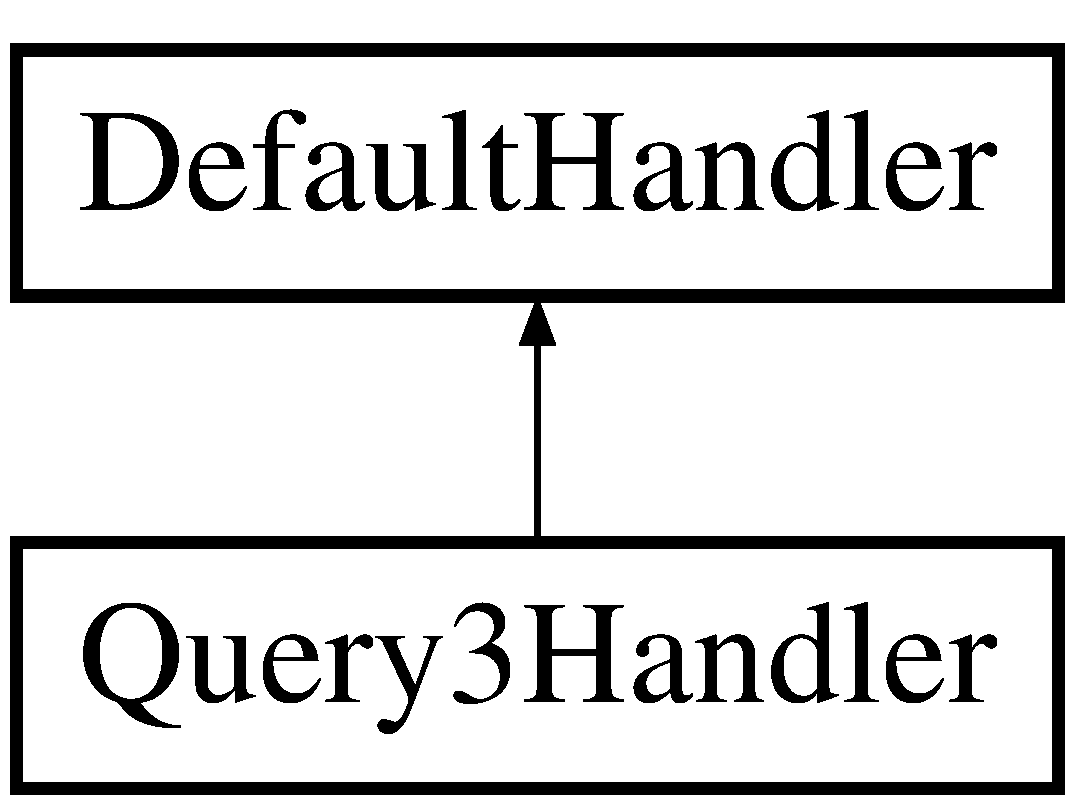
\includegraphics[height=2.000000cm]{class_query3_handler}
\end{center}
\end{figure}


The documentation for this class was generated from the following file\+:\begin{DoxyCompactItemize}
\item 
src/\hyperlink{_query3_handler_8java}{Query3\+Handler.\+java}\end{DoxyCompactItemize}

\hypertarget{class_result_panel}{}\section{Result\+Panel Class Reference}
\label{class_result_panel}\index{Result\+Panel@{Result\+Panel}}
\subsection*{Public Member Functions}
\begin{DoxyCompactItemize}
\item 
\hyperlink{class_result_panel_a1f0864074da52caf14581a14b2574d48}{Result\+Panel} ()
\item 
J\+Scroll\+Pane \hyperlink{class_result_panel_ace0f4c9bd2c1ddadc0e0484ac9da3d2b}{get\+Pane} ()
\end{DoxyCompactItemize}
\subsection*{Static Public Member Functions}
\begin{DoxyCompactItemize}
\item 
static void \hyperlink{class_result_panel_a46714631f37ba703978bdd94e6a666d3}{update\+Data} (Object\mbox{[}$\,$\mbox{]}\mbox{[}$\,$\mbox{]} \+\_\+data, String\mbox{[}$\,$\mbox{]} col\+Data)
\item 
static void \hyperlink{class_result_panel_a91bbedbe216c200121a25a629bdc6d2f}{update\+Table} ()
\end{DoxyCompactItemize}
\subsection*{Private Member Functions}
\begin{DoxyCompactItemize}
\item 
void \hyperlink{class_result_panel_a42092133d8e2f6819a8f1ee557b2fc1f}{build\+Gui} ()
\end{DoxyCompactItemize}
\subsection*{Private Attributes}
\begin{DoxyCompactItemize}
\item 
J\+Scroll\+Pane \hyperlink{class_result_panel_aa9b24b254e779baf6679dbbc6af4fe38}{pane}
\end{DoxyCompactItemize}
\subsection*{Static Private Attributes}
\begin{DoxyCompactItemize}
\item 
static J\+Table \hyperlink{class_result_panel_a7efcc61cd33b439bb4a4ce365a05fcd9}{table}
\item 
static Object \mbox{[}$\,$\mbox{]}\mbox{[}$\,$\mbox{]} \hyperlink{class_result_panel_ac748be7e13e72b23ee1b7486c71e4400}{row\+Data}
\item 
static String \hyperlink{class_result_panel_ad2246ab66ef229df1e6d89d570e19364}{column\+Names} \mbox{[}$\,$\mbox{]} = \{ \char`\"{}title\char`\"{},\char`\"{}author\char`\"{} ,\char`\"{}year\char`\"{}, \char`\"{}volume\char`\"{},\char`\"{}pages\char`\"{},\char`\"{}journal/booktitle\char`\"{},\char`\"{}url\char`\"{} \}
\end{DoxyCompactItemize}


\subsection{Constructor \& Destructor Documentation}
\hypertarget{class_result_panel_a1f0864074da52caf14581a14b2574d48}{}\label{class_result_panel_a1f0864074da52caf14581a14b2574d48} 
\index{Result\+Panel@{Result\+Panel}!Result\+Panel@{Result\+Panel}}
\index{Result\+Panel@{Result\+Panel}!Result\+Panel@{Result\+Panel}}
\subsubsection{\texorpdfstring{Result\+Panel()}{ResultPanel()}}
{\footnotesize\ttfamily Result\+Panel.\+Result\+Panel (\begin{DoxyParamCaption}{ }\end{DoxyParamCaption})}



\subsection{Member Function Documentation}
\hypertarget{class_result_panel_a42092133d8e2f6819a8f1ee557b2fc1f}{}\label{class_result_panel_a42092133d8e2f6819a8f1ee557b2fc1f} 
\index{Result\+Panel@{Result\+Panel}!build\+Gui@{build\+Gui}}
\index{build\+Gui@{build\+Gui}!Result\+Panel@{Result\+Panel}}
\subsubsection{\texorpdfstring{build\+Gui()}{buildGui()}}
{\footnotesize\ttfamily void Result\+Panel.\+build\+Gui (\begin{DoxyParamCaption}{ }\end{DoxyParamCaption})\hspace{0.3cm}{\ttfamily [private]}}

\hypertarget{class_result_panel_ace0f4c9bd2c1ddadc0e0484ac9da3d2b}{}\label{class_result_panel_ace0f4c9bd2c1ddadc0e0484ac9da3d2b} 
\index{Result\+Panel@{Result\+Panel}!get\+Pane@{get\+Pane}}
\index{get\+Pane@{get\+Pane}!Result\+Panel@{Result\+Panel}}
\subsubsection{\texorpdfstring{get\+Pane()}{getPane()}}
{\footnotesize\ttfamily J\+Scroll\+Pane Result\+Panel.\+get\+Pane (\begin{DoxyParamCaption}{ }\end{DoxyParamCaption})}

\hypertarget{class_result_panel_a46714631f37ba703978bdd94e6a666d3}{}\label{class_result_panel_a46714631f37ba703978bdd94e6a666d3} 
\index{Result\+Panel@{Result\+Panel}!update\+Data@{update\+Data}}
\index{update\+Data@{update\+Data}!Result\+Panel@{Result\+Panel}}
\subsubsection{\texorpdfstring{update\+Data()}{updateData()}}
{\footnotesize\ttfamily static void Result\+Panel.\+update\+Data (\begin{DoxyParamCaption}\item[{Object}]{\+\_\+data\mbox{[}$\,$\mbox{]}\mbox{[}$\,$\mbox{]},  }\item[{String \mbox{[}$\,$\mbox{]}}]{col\+Data }\end{DoxyParamCaption})\hspace{0.3cm}{\ttfamily [static]}}

\hypertarget{class_result_panel_a91bbedbe216c200121a25a629bdc6d2f}{}\label{class_result_panel_a91bbedbe216c200121a25a629bdc6d2f} 
\index{Result\+Panel@{Result\+Panel}!update\+Table@{update\+Table}}
\index{update\+Table@{update\+Table}!Result\+Panel@{Result\+Panel}}
\subsubsection{\texorpdfstring{update\+Table()}{updateTable()}}
{\footnotesize\ttfamily static void Result\+Panel.\+update\+Table (\begin{DoxyParamCaption}{ }\end{DoxyParamCaption})\hspace{0.3cm}{\ttfamily [static]}}



\subsection{Member Data Documentation}
\hypertarget{class_result_panel_ad2246ab66ef229df1e6d89d570e19364}{}\label{class_result_panel_ad2246ab66ef229df1e6d89d570e19364} 
\index{Result\+Panel@{Result\+Panel}!column\+Names@{column\+Names}}
\index{column\+Names@{column\+Names}!Result\+Panel@{Result\+Panel}}
\subsubsection{\texorpdfstring{column\+Names}{columnNames}}
{\footnotesize\ttfamily String Result\+Panel.\+column\+Names\mbox{[}$\,$\mbox{]} = \{ \char`\"{}title\char`\"{},\char`\"{}author\char`\"{} ,\char`\"{}year\char`\"{}, \char`\"{}volume\char`\"{},\char`\"{}pages\char`\"{},\char`\"{}journal/booktitle\char`\"{},\char`\"{}url\char`\"{} \}\hspace{0.3cm}{\ttfamily [static]}, {\ttfamily [private]}}

\hypertarget{class_result_panel_aa9b24b254e779baf6679dbbc6af4fe38}{}\label{class_result_panel_aa9b24b254e779baf6679dbbc6af4fe38} 
\index{Result\+Panel@{Result\+Panel}!pane@{pane}}
\index{pane@{pane}!Result\+Panel@{Result\+Panel}}
\subsubsection{\texorpdfstring{pane}{pane}}
{\footnotesize\ttfamily J\+Scroll\+Pane Result\+Panel.\+pane\hspace{0.3cm}{\ttfamily [private]}}

\hypertarget{class_result_panel_ac748be7e13e72b23ee1b7486c71e4400}{}\label{class_result_panel_ac748be7e13e72b23ee1b7486c71e4400} 
\index{Result\+Panel@{Result\+Panel}!row\+Data@{row\+Data}}
\index{row\+Data@{row\+Data}!Result\+Panel@{Result\+Panel}}
\subsubsection{\texorpdfstring{row\+Data}{rowData}}
{\footnotesize\ttfamily Object \mbox{[}$\,$\mbox{]}\mbox{[}$\,$\mbox{]} Result\+Panel.\+row\+Data\hspace{0.3cm}{\ttfamily [static]}, {\ttfamily [private]}}

{\bfseries Initial value\+:}
\begin{DoxyCode}
=\{
            \{\textcolor{stringliteral}{" "},\textcolor{stringliteral}{" "},\textcolor{stringliteral}{" "},\textcolor{stringliteral}{" "},\textcolor{stringliteral}{" "},\textcolor{stringliteral}{" "},\textcolor{stringliteral}{" "}\}
    \}
\end{DoxyCode}
\hypertarget{class_result_panel_a7efcc61cd33b439bb4a4ce365a05fcd9}{}\label{class_result_panel_a7efcc61cd33b439bb4a4ce365a05fcd9} 
\index{Result\+Panel@{Result\+Panel}!table@{table}}
\index{table@{table}!Result\+Panel@{Result\+Panel}}
\subsubsection{\texorpdfstring{table}{table}}
{\footnotesize\ttfamily J\+Table Result\+Panel.\+table\hspace{0.3cm}{\ttfamily [static]}, {\ttfamily [private]}}



The documentation for this class was generated from the following file\+:\begin{DoxyCompactItemize}
\item 
src/\hyperlink{_result_panel_8java}{Result\+Panel.\+java}\end{DoxyCompactItemize}

\chapter{File Documentation}
\hypertarget{_data_8java}{}\section{Data.\+java File Reference}
\label{_data_8java}\index{Data.\+java@{Data.\+java}}
\subsection*{Classes}
\begin{DoxyCompactItemize}
\item 
class \hyperlink{class_data}{Data}
\end{DoxyCompactItemize}

\hypertarget{_database_8java}{}\section{src/\+Database.java File Reference}
\label{_database_8java}\index{src/\+Database.\+java@{src/\+Database.\+java}}
\subsection*{Classes}
\begin{DoxyCompactItemize}
\item 
class \hyperlink{class_database}{Database}
\end{DoxyCompactItemize}

\hypertarget{main_class_8java}{}\section{src/main\+Class.java File Reference}
\label{main_class_8java}\index{src/main\+Class.\+java@{src/main\+Class.\+java}}
\subsection*{Classes}
\begin{DoxyCompactItemize}
\item 
class \hyperlink{classmain_class}{main\+Class}
\end{DoxyCompactItemize}

\hypertarget{my_frame_8java}{}\section{my\+Frame.\+java File Reference}
\label{my_frame_8java}\index{my\+Frame.\+java@{my\+Frame.\+java}}
\subsection*{Classes}
\begin{DoxyCompactItemize}
\item 
class \hyperlink{classmy_frame}{my\+Frame}
\end{DoxyCompactItemize}

\hypertarget{my_panel_8java}{}\section{my\+Panel.\+java File Reference}
\label{my_panel_8java}\index{my\+Panel.\+java@{my\+Panel.\+java}}
\subsection*{Classes}
\begin{DoxyCompactItemize}
\item 
class \hyperlink{classmy_panel}{my\+Panel}
\end{DoxyCompactItemize}

\hypertarget{my_query1_panel_8java}{}\section{my\+Query1\+Panel.\+java File Reference}
\label{my_query1_panel_8java}\index{my\+Query1\+Panel.\+java@{my\+Query1\+Panel.\+java}}
\subsection*{Classes}
\begin{DoxyCompactItemize}
\item 
class \hyperlink{classmy_query1_panel}{my\+Query1\+Panel}
\end{DoxyCompactItemize}

\hypertarget{my_query2_panel_8java}{}\section{src/my\+Query2\+Panel.java File Reference}
\label{my_query2_panel_8java}\index{src/my\+Query2\+Panel.\+java@{src/my\+Query2\+Panel.\+java}}
\subsection*{Classes}
\begin{DoxyCompactItemize}
\item 
class \hyperlink{classmy_query2_panel}{my\+Query2\+Panel}
\end{DoxyCompactItemize}

\hypertarget{my_query3_panel_8java}{}\section{my\+Query3\+Panel.\+java File Reference}
\label{my_query3_panel_8java}\index{my\+Query3\+Panel.\+java@{my\+Query3\+Panel.\+java}}
\subsection*{Classes}
\begin{DoxyCompactItemize}
\item 
class \hyperlink{classmy_query3_panel}{my\+Query3\+Panel}
\end{DoxyCompactItemize}

\hypertarget{_parser_8java}{}\section{Parser.\+java File Reference}
\label{_parser_8java}\index{Parser.\+java@{Parser.\+java}}
\subsection*{Classes}
\begin{DoxyCompactItemize}
\item 
class \hyperlink{class_parser}{Parser}
\item 
class {\bfseries Parser.\+Progress\+Bar}
\end{DoxyCompactItemize}

\hypertarget{_query1_handler_8java}{}\section{Query1\+Handler.\+java File Reference}
\label{_query1_handler_8java}\index{Query1\+Handler.\+java@{Query1\+Handler.\+java}}
\subsection*{Classes}
\begin{DoxyCompactItemize}
\item 
class \hyperlink{class_query1_handler}{Query1\+Handler}
\end{DoxyCompactItemize}

\hypertarget{_query2_handler_8java}{}\section{Query2\+Handler.\+java File Reference}
\label{_query2_handler_8java}\index{Query2\+Handler.\+java@{Query2\+Handler.\+java}}
\subsection*{Classes}
\begin{DoxyCompactItemize}
\item 
class \hyperlink{class_query2_handler}{Query2\+Handler}
\end{DoxyCompactItemize}

\hypertarget{_query3_handler_8java}{}\section{src/\+Query3\+Handler.java File Reference}
\label{_query3_handler_8java}\index{src/\+Query3\+Handler.\+java@{src/\+Query3\+Handler.\+java}}
\subsection*{Classes}
\begin{DoxyCompactItemize}
\item 
class \hyperlink{class_query3_handler}{Query3\+Handler}
\end{DoxyCompactItemize}

\hypertarget{_result_panel_8java}{}\section{src/\+Result\+Panel.java File Reference}
\label{_result_panel_8java}\index{src/\+Result\+Panel.\+java@{src/\+Result\+Panel.\+java}}
\subsection*{Classes}
\begin{DoxyCompactItemize}
\item 
class \hyperlink{class_result_panel}{Result\+Panel}
\end{DoxyCompactItemize}

%--- End generated contents ---

% Index
\backmatter
\newpage
\phantomsection
\clearemptydoublepage
\addcontentsline{toc}{chapter}{Index}
\printindex

\end{document}
